\chapter{Implementation}
\label{ch:implementation}

Die Implementation der verschiedenen Deep-Learning Bilderkennungsmethoden erfolgte durch die Verwendung des Ultralytics YOLO \cite{Jocher_Ultralytics_YOLO_2023} Frameworks und der Eigenimplementation der U-Net \cite{ronneberger2015unetconvolutionalnetworksbiomedical} Architektur. Alle folgenden Modelle wurden auf einer NVIDIA GeForce RTX 3090 mit 24252 MiB Grafikkartenspeicher trainiert.

\section{Ultralytics YOLO}
Für die Extraktion von Diagrammen aus Texten, Schwierigkeitsklassifizierung von Liniendiagrammen und Instanzsegmentation der Wertelinien wurde das Ultralytics YOLO Framework verwendet. Es basiert auf der YOLO (You Only Look Once) Architektur, welche erstmal 2015 \cite{redmon2016lookonceunifiedrealtime} veröffentlicht wurde, und seit dem zehn Versionsiterationen durchlief. Unterstützt werden verschiedene Bild- und Videoerkennungsaufgaben, wie die Erkennung (detection), Segmentierung (segmentation), Posenschätzung (pose detection), Verfolgung (tracking) und Klassifizierung (classification). Das Ultralytics YOLO Framework ist anfängerfreundlich, die Verwendung erfolgt einfach, verfügt man bereits über einen annotierten Datensatz, kann mit lediglich einem Konsolenbefehl der Trainingsprozess des eigenen Modells gestartet werden. Ebenfalls verfügt es über der automatischen Datenagumentation während des Trainingsvorgangs und der Evaluation verschiedener Metriken des trainierenden und trainierten Modells.
\\
Ultralytics stellt zu dem Großteil der zehn YOLO Architekturen bereits vortrainierte herunterladbare Modelle bereit. Für das Vortrainieren der Objekterkennung, Klassifizierung und Instanzsegmentation wurde der COCO \cite{lin2015microsoftcococommonobjects} Datensatz verwendet, welcher aus über 200.000 Bildern besteht und  eingeteilt wurde auf 80 Objektklassen.

Diese werden außerdem in verschiedene Modellgrößen angeboten, sodass die Möglichkeit besteht zwischen Invarianzgeschwindigkeit, benötigte Gleitkommaoperationsleistungsfähigkeiten und verwendbaren Grafikkartenspeicher abwegegen zu können.
\\
Es wurden verschiedene YOLO Modelle verwendet, an denen jedoch keine Architekturänderungen vorgenommen wurden.
Sofern im Weiteren nicht explizit angegeben, wurden die Grundeinstellungen des Ultralytics YOLO Frameworks benutzt. Die genaue Anzahl der Trainingsepochen variierte zwischen den einzelnen Trainingsvorgängen, da bei allen die Geduldseinstellung (patience) von 100 Epochen verwendet wurde. Um die Überanpassung (over-fitting) an den Trainingsdatensatz zu vermeiden, wird mit diesem Geduldsparameter das Training vorzeitig abgebrochen, solange in den letzten beliebigen Epochen das trainierende Modell keine Verbesserungen der Validationsmetriken aufweisen konnte.

\subsection{Objekterkennung zur Extraktion von Diagrammen aus Texten}
\label{ch:objectdetection}

Für die Erkennung aller Diagrammen in den Vollseitscans wurde das YOLOv9e Modell verwendet.
\\
Zuerst wurde es auf den in \ref{ch:chartbank} beschreibenen, selbst erstellten DocBank Datensatz vortrainiert (pre-trained) und danach auf den Datensatz aus \ref{ch:scanbank}, der historischen Wirtschaftsscans, feintrainiert (fine-tuned). Beide Datensätze wurden mit der häufig verwendeten 80-20 Aufteilung differenziert. In diesem Fall werden 80\% des Datensatzes für das Trainieren und 20\% für das Evaluieren des Modells benutzt. Die hierbei 20\% des Evaluationssets bestehen aus Daten, welche das Modell vor dem Zeitpunkt noch nie gesehenen hat und dementsprechend unbekannt sind.
\\
Es wurde die Bildgröße von 1024x1024 Pixel verwendet und eine Batchgröße von 7 gewählt, da für eine höhere Batchgröße die verwendete Grafikkarte über ungenügend viel Speicher verfügte. Die von den Grundeinstellungen geänderten Parametern der Datenaugmentierung, mitsamt ihrer jeweiligen Wahrscheinlichkeiten, bestanden aus:

\begin{itemize}[itemsep=0pt, topsep=0pt]
    \item Farbmanipulation im HSV-Farbraum: Hue (1.0), Sättigung (1.0) und Helligkeit (0.5)
    \item BGR-Kanaländerung (0.5)
    \item Skalierung (1.0)
    \item Vertikales Spiegeln (0.1)
    \item Überlagern von Bildern (Mixup, 1.0)
\end{itemize}

Gewählt wurden diese Augmentierungstechniken mit dem Ziel die universelle Erkennungsfähigkeiten des trainierted Modells zu stärken. Farbmanipulationen helfen dem Modell zuversichtlichere Vorhersagen auf einer breiten Spanne unterschiedlicher Papierhintergründe zu treffen, beziehungsweise Diagramme mit willkürlichen Farben besser zu erkennen.

\clearpage


\subsection{Klassifizierung zur Schwierigkeitsbestimmung von Liniendiagrammen}

Der Trainingsvorgang der Schwierigkeitsklassifizierung der Liniendiagrammen folgte ähnlich der Objekterkennung aus \ref{ch:objectdetection}. Da hier das gewählte YOLOv8m-cls Modell nur Vorhersagen über bereits extrahierte Diagramme machen muss und nicht mehr über Vollseitscans, wurde die Bildgröße auf 640x640 Pixel reduziert. Im Vergleich zu der vorherigen Objekterkennung konnten keine Verbesserungen der Verwendung eines größeren Modells beobachtet werden, weshlab für die Klassifizierung lediglich das Modell mittlerer Größe gewählt wurde. Die Batchgröße dagegen wurde auf 16 erhöht und ebenfalls wurde wieder der Trainingsprozess durch den Geduldsparameter von 100 beendet, anstatt durch eine festgelegte Epochenbegrenzung. Die veränderten Augmentierungstechniken, sowie deren Parameter, bestanden aus:

\begin{itemize}[itemsep=0pt, topsep=0pt]
    \item Farbmanipulation im HSV-Farbraum: Hue (1.0), Sättigung (1.0) und Helligkeit (0.5)
    \item BGR-Kanaländerung (0.5)
    \item Vertikales Spiegeln (0.1)
    \item Rotation ($\pm$5°)
    \item Scherung ($\pm$5°)
    \item Zufälliges Löschen (1.0)
\end{itemize}

Auch wenn das Löschen zufälliger Bereiche im Bild möglicherweise kontraproduktiv wirkt, erziehlte die Verwendung dieser Technik zu besseren Ergebnissen, weshalb sie mit einbezogen wurde. Die restlichen Augmentierungen wurden für die breitere Diagrammsvarianz gewählt.

\begin{figure}[H]
    \centering
    \captionsetup{width=.75\linewidth}
    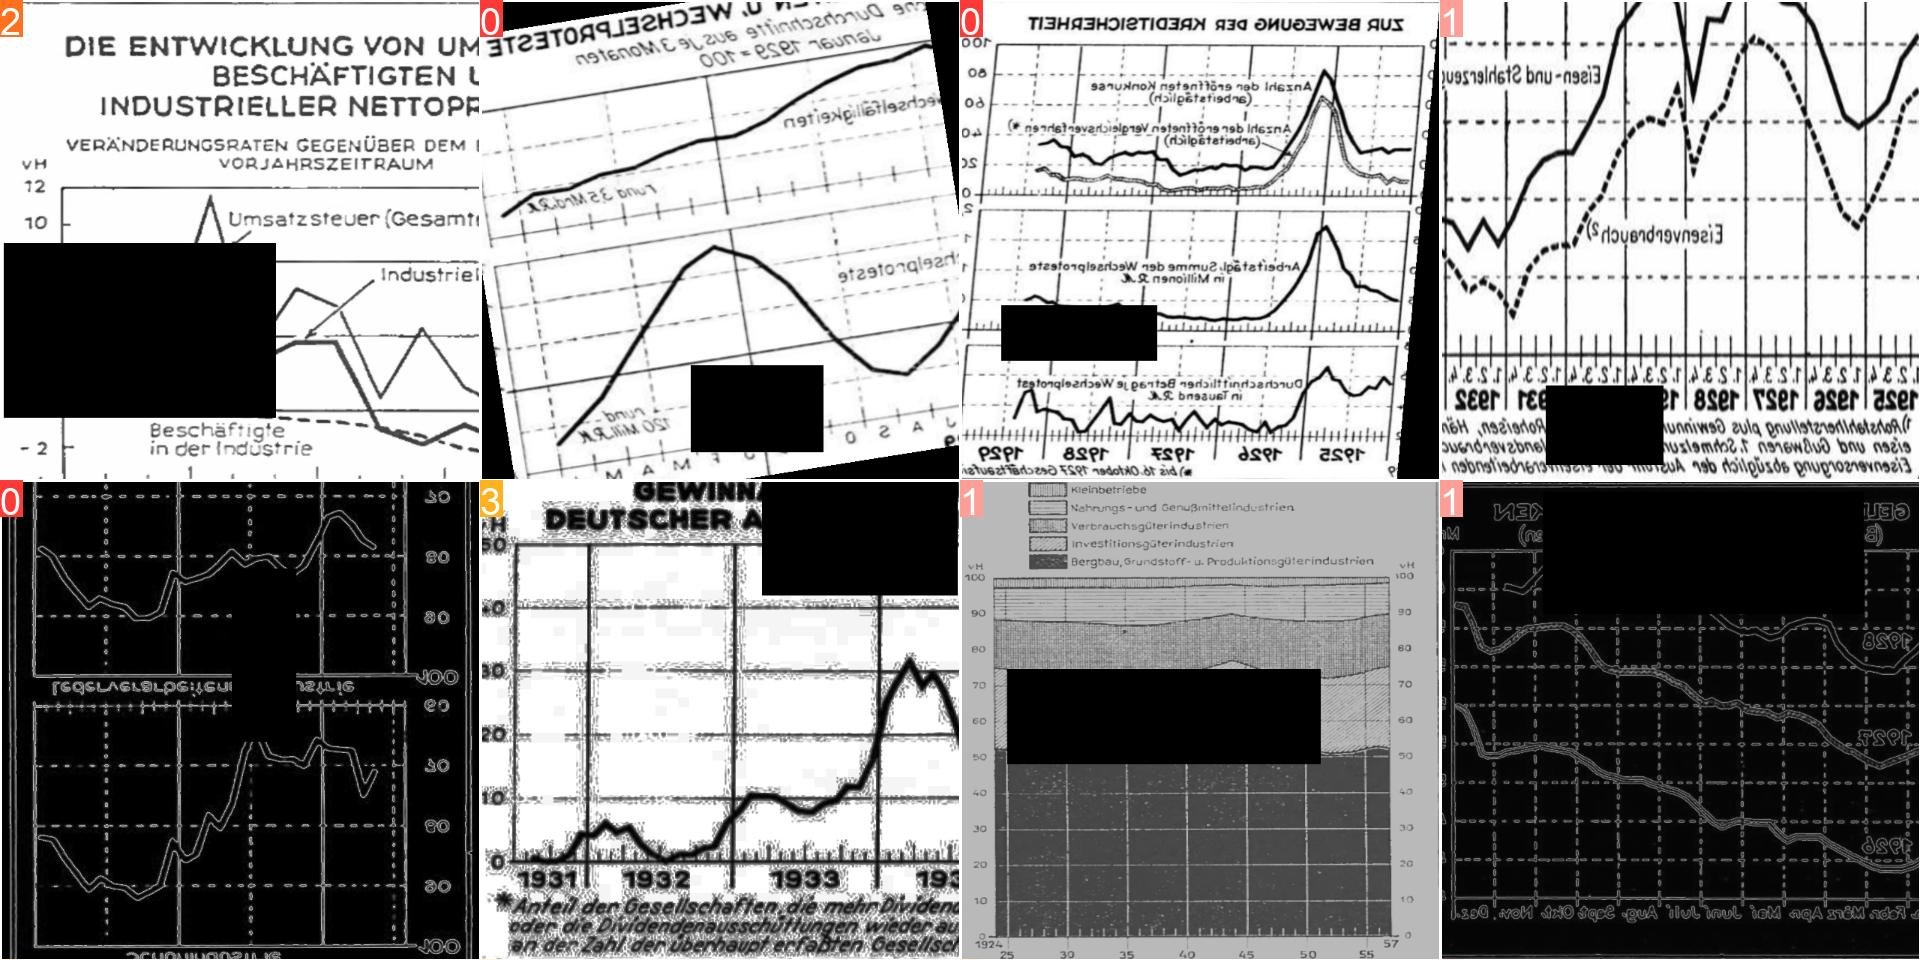
\includegraphics[width=.75\textwidth]{Implementation/img/classify_train_batch.jpg}
    \caption{\hbadness=10000 Augmentierter Trainingsbatch der Klassifizierung}
    \label{fig:classify_train_batch}
\end{figure}

Desweiteren wurde dieser beschriebene Trainingsprozess erneut auf der anderen Version, des in \ref{ch:linebank} beschriebenen, Datensatzes mit der Vereinigung der sich überlappenden und nicht überlappenden Wertelinien in die gemeinsame Klasse mehrerer Wertelinien trainiert.

\subsection{Instanzsegmentation von Wertelinien in Liniendiagrammen}

Die Instanzsegmentation durch Ultralytics YOLO erfolgte mithilfe der in \ref{ch:genlines} und \ref{ch:lines} definierten Datensätze der Wertelinien synthetischer und historischer Liniendiagramme. Wie zuvor beschrieben wurden diese zuerst in das, von dem Framework benötigte, Polygonannotationsformat konvertiert. Hierzu wurde Python 3.10.12 in Verbindung mit der Bildverarbeitungsbibliothek OpenCV \cite{opencv_library} verwendet. Die Korrektheit der Konvertation von den Binärmasken in Polygonform wurde durch den von Ultralytics erstellten Trainingsbatches, als auch durch Auswertung mithilfe der Annotationswebseite Roboflow \cite{dwyer2024roboflow} überprüft werden. Im Anschluss konnte das YOLOv8x-seg Model mit einer Bildgröße von 512x512 Pixel und Batchgröße von 16 trainiert werden. Der Trainingsprozess verlief erneut in zwei Schritten.
Diese Parameter wurden für sowohl das Vortrainieren auf den synthetischen, als auch das Feintrainieren auf den  historischen Liniendiagrammen gewählt. Ebenfalls wurden für beie Trainingsprozesse dieselben Augmentierungstechniken verwendet:

\begin{itemize}[itemsep=0pt, topsep=0pt]
    \item Farbmanipulation im HSV-Farbraum: Hue (1.0), Sättigung (1.0) und Helligkeit (0.5)
    \item BGR-Kanaländerung (0.5)
    \item Vertikales Spiegeln (0.5)
    \item Rotation ($\pm$90°)
    \item Zufälliges Löschen (0.7)
    \item Überlagern von Bildern (Mixup, 0.5)
\end{itemize}

\begin{figure}[H]
    \centering
    \captionsetup{width=.75\linewidth}
    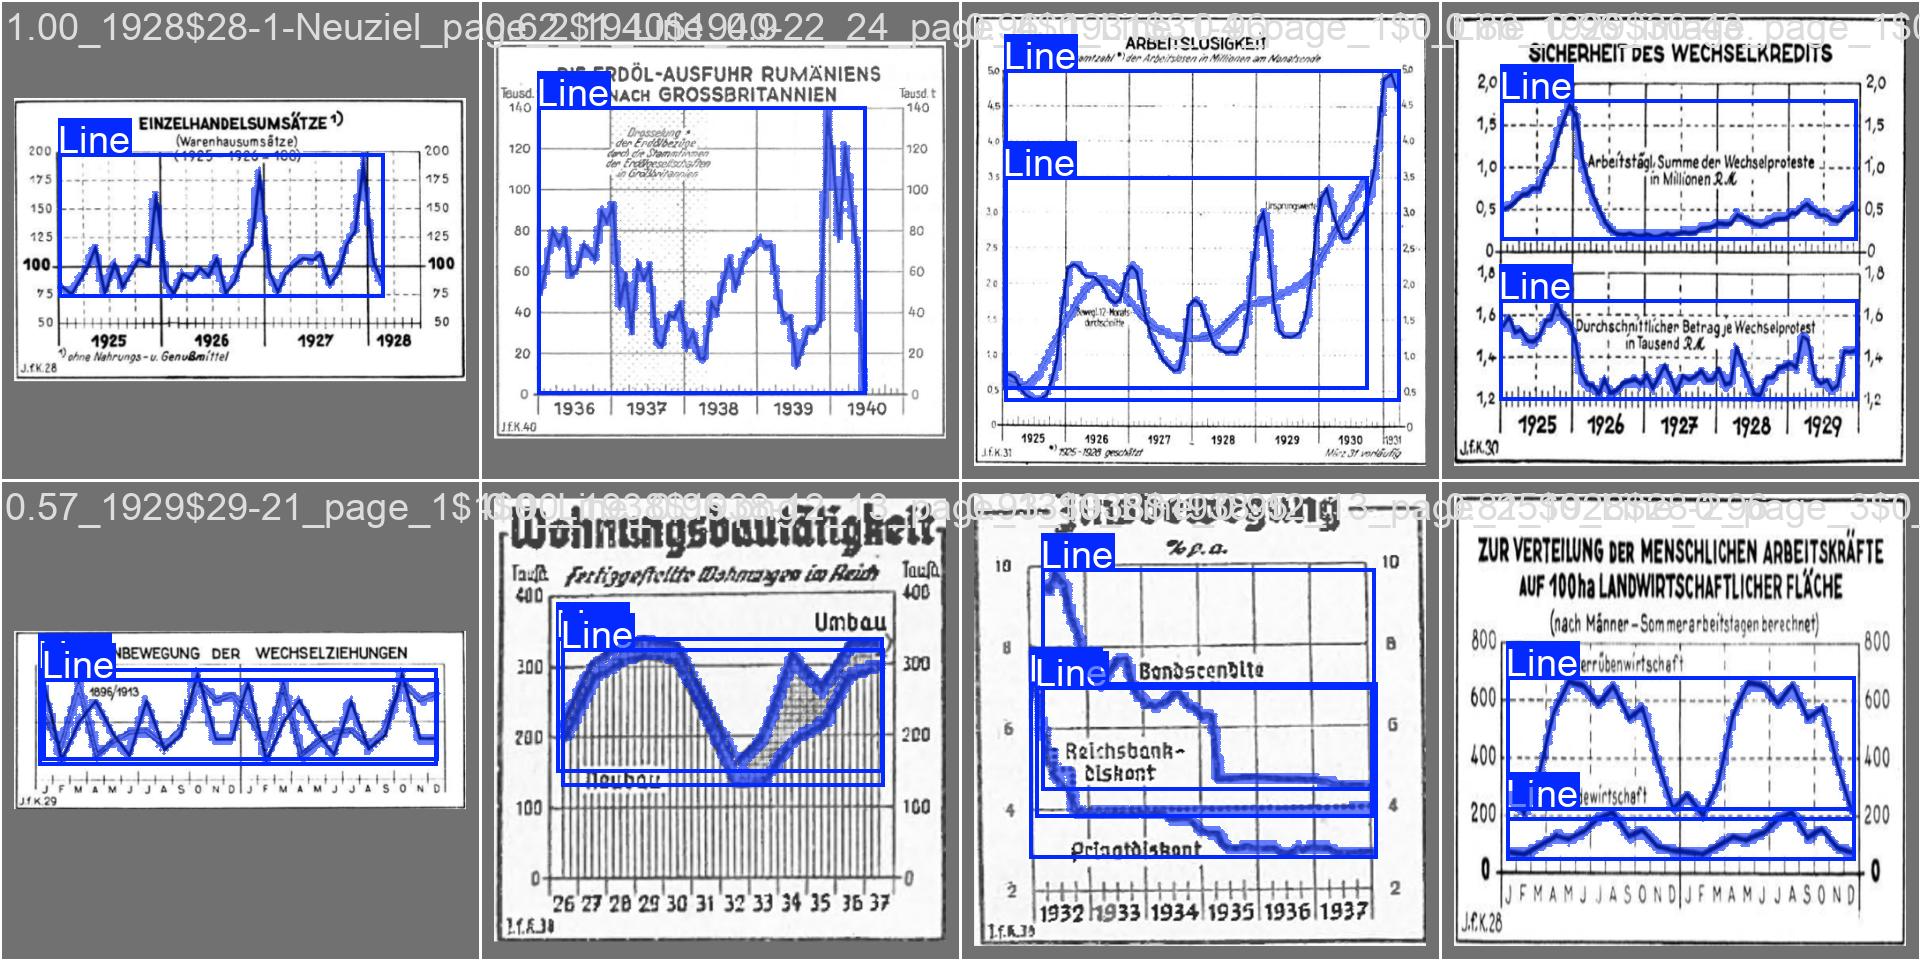
\includegraphics[width=.75\textwidth]{Implementation/img/instance_annotated.png}
    \caption{\hbadness=10000 Annotierte Wertelinien der Liniendiagrammen zur Instanzsegmentation}
    \label{fig:instance_annotated}
\end{figure}

Hier wurden stärkere Augmentierungstechniken gewählt, da Wertelinien unabhängig von Positionskontexten ausfindig gemacht werden müssen, weshlab additionell höhere Rotations- und Spiegelungsparameter verwendet wurden.


\section{U-Net: Semantische Segmentation von Wertelinien}
\label{ch:unet}

Als Alternative zur Instanzsegmentation wurde ebenfalls die semantische Segmentation durch die Eigenimplementation der U-Net Architektur verwirklicht. Diese wurde speziell für die medizinisch Bildsegmentierung entwickelt und zeichnet sich besonders bei einer limitierten Anzahl von Trainingsdaten aus. Die Architektur des CNNs (convolutional neural network) kombiniert Encoder- und Decoderpfade mit Skip-Verbindungen um so präzise Segmentationsergebnisse zu erziehlen.
\\
Implementiert wurde die Datenvorverarbeitung, das Modelltraining und die Evaluation mithilfe der Keras 3 API \cite{chollet2015keras}. Für die Augmentierung der Trainingsdaten wurde die Bibliothek Albumentations \cite{info11020125} genutzt. Lediglich der Code der U-Net Architektur selbst wurde in Form des Vanilla U-Nets \cite{zak2024kerasunet} übernommen.
\\
Der Ablauf des U-Net Trainings durchlief wie folgt:
Zuerst wurde der Datensatz mithilfe verfügbarer Bibliotheksfunktionen eingelesen. Im Fall der Binärmasken wurde der Schwellenwert (threshold) von 30\% genutzt. Nach der Deklaration der Modellarchitektur wurde die Datenagumentation definiert. Folgende Augmentierungstechniken wurden verwendet:

\begin{itemize}[itemsep=0pt, topsep=0pt]
    \item Spiegeln entlang der horizontalen Achse (\texttt{A.HorizontalFlip}, \texttt{p=0.5})
    \item Spiegeln entlang der vertikalen Achse (\texttt{A.VerticalFlip}, \texttt{p=0.5})
    \item Drehung des Bildes (\texttt{A.RandomRotate90}, \texttt{p=0.5})
    \item Vertauschen von Breite und Höhe (\texttt{A.Transpose}, \texttt{p=0.5})
    \item Ausschneiden und Skalieren auf eine feste Größe (\texttt{A.RandomResizedCrop}, \texttt{height=512}, \texttt{width=512}, \texttt{scale=(0.8, 1.0)}, \texttt{p=0.5})
    \item Zuschneiden auf eine feste Größe vom Zentrum aus (\texttt{A.CenterCrop}, \texttt{height=512}, \texttt{width=512}, \texttt{p=0.5})
    \item Ausschneiden eines Bereichs des Bildes basierend auf der Maske (\texttt{A.CropNonEmptyMaskIfExists}, \texttt{height=512}, \texttt{width=512}, \texttt{p=0.5})
    \item Zufälliges Löschen von Bereichen (\texttt{A.CoarseDropout}, \texttt{max\_holes=8}, \texttt{max\_height=64}, \texttt{max\_width=64}, \texttt{p=0.5})
    \item Anpassung von Helligkeit und Kontrast (\texttt{A.RandomBrightnessContrast}, \texttt{p=0.5})
    \item Anwendung von Gamma-Korrektur (\texttt{A.RandomGamma}, \texttt{p=0.5})
    \item Zufälliges Mischen der Farbkanäle (\texttt{A.ChannelShuffle}, \texttt{p=0.5})
    \item Umkehren der Pixelwerte (\texttt{A.Solarize}, \texttt{threshold=128}, \texttt{p=0.1})
    \item Vollständiges Invertieren der Farbwerte (\texttt{A.InvertImg}, \texttt{p=0.1})
    \item Skalieren auf die maximale Größe entlang der längsten Kante (\texttt{A.LongestMaxSize}, \texttt{max\_size=512}, \texttt{p=1.0})
    \item Auffüllen auf eine Mindestgröße mit konstantem Rand (\texttt{A.PadIfNeeded}, \texttt{min\_height=512}, \texttt{min\_width=512}, \texttt{border\_mode=cv2.BORDER\_CONSTANT}, \texttt{value=0}, \texttt{p=1.0})
    \item Überlagern mit einem anderen Bild (\texttt{A.MixUp}, \texttt{p=1.0}, \texttt{alpha=0.7})
\end{itemize}

Es wurde eingerichtet, dass die Trainingsbilder samt ihrer zugehörigen Binärmasken jeweils pro Batch neu augmentiert werden. Der Validationsdatensatz dagegen wurde unaugmentiert verarbeitet. Durch Abspeichern der einzelnen Bilderbatches konnte der fehlerfreie Augmentierungsablauf manuell verifiziert werden.

\begin{figure}[H]
    \centering
    \captionsetup{width=.75\linewidth}
    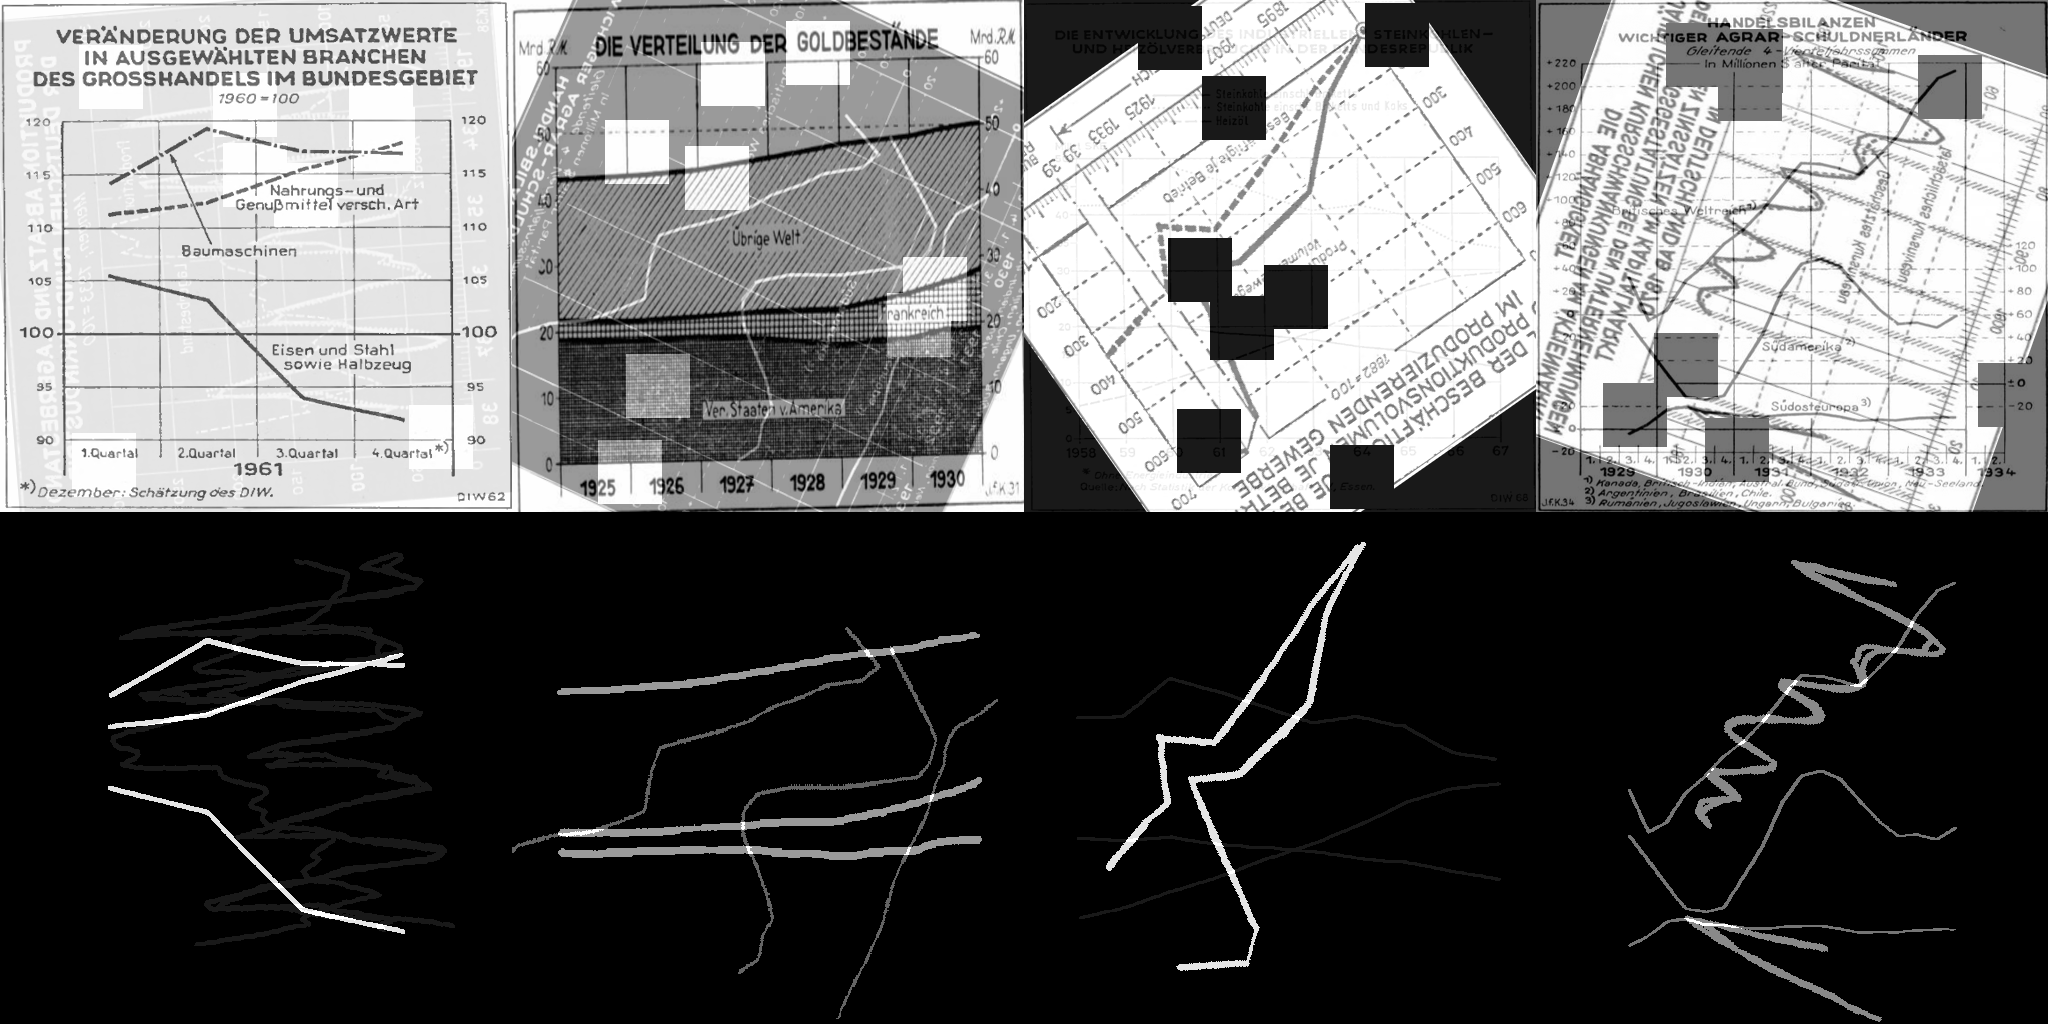
\includegraphics[width=.75\textwidth]{Implementation/img/unet_training.png}
    \caption{\hbadness=10000 Augmentierter Trainingsbatch inklusive der zugehörigen Binärmasken}
    \label{fig:unet_training}
\end{figure}

Nach diesem Implementationsschritt konnte der Trainingsprozess gestartet werden. Hierfür wurde ebenfalls, die für die Grafikkarte größtmöglichste Batchgröße von 7 verwendet, und ein Geduldsparameter von 100 Epochen genutzt, welcher das Training zum frühzeitigen Abbrechen (early stopping) führt. Als Überwachungsmetrik (monitor) dafür wurde der Trainingsverlust (training loss) gewählt; sobald dieser über die bestimmte Anzahl an Epochen nicht unterschritten wurde, beendet das Training vorzeitig. Aufgrund der Minimierungsoptimierung des verwendeten Adam Optimierers (optimizer) \cite{kingma2017adammethodstochasticoptimization} wurde dieser Trainings Loss als Negativ des Dice-Sørensen-Koeffizient (dice score) festgelegt, welcher ebenfalls als Validationsfunktion dient. Der Dice Score misst die Überlappung zwischen der Vorhersage und der Ground Truth, wobei ein Wert von 1 eine perfekte Übereinstimmung und 0 keine Übereinstimmung bedeutet. Als Learnrate (learning rate) wurde 0.0001 und als Dropout-Rate 0.0 gewählt. Für die genannten Validations- und Verlustfunktionen wurden folgende Formeln verwendet:

% Dice Score Function
\begin{equation}
    \text{Dice Score}(y_{\text{true}}, y_{\text{pred}}) = \frac{2 \cdot \sum_{i} (y_{\text{true}_i} \cdot y_{\text{pred}_i}) + 1}{\sum_{i} y_{\text{true}_i} + \sum_{i} y_{\text{pred}_i} + 1} \nonumber
\end{equation}

% Dice Loss Function
\begin{equation}
    \text{Dice Loss}(y_{\text{true}}, y_{\text{pred}}) = -\text{Dice Score}(y_{\text{true}}, y_{\text{pred}}) \nonumber
\end{equation}

Hierbei steht $y_{\text{true}}$ für die Grundwahrheiten und $y_{\text{pred}}$ für die Modellvorhersagen. Der Index $i$ läuft über alle Pixel der Bilder. Die Addition von 1 im Zähler und Nenner dient der numerischen Stabilität.


\section{Numerische Auswertung von Liniendiagrammen in Tabellenform}

Um die historischen Liniendiagramme in Tabellenform auswerten zu können wurde die vorherig beschriebene U-Net Segmentierung mitbenutzt. Die generelle Idee des Auswertungsalgorithmus besteht aus der Kombination der, durch die implementierte Segmentierung möglichgemachte, Wertelinienerkennung und einer optischen Schriftzeichenerkennung (optical character recognition; OCR), aus welcher unter anderem Achsenbeschriftungen und deren numerischen Kontext extrahiert werden können. Umgesetzt wurde dieser Algorithmus ebenfalls der Programmiersprache Python. Im Folgenden wird die Funktionsweise des zweigeteilten Algorithmus im Nähren beschreiben.

\subsection{Extraktion der segmentierten Wertelinien}

Aufgrund der, später sichtlich gemachten, souveräneren Ergebnisse des U-Nets im Vergleich mit dem Ultralytics YOLO Segmentierungsmodell, wurde dieses für die Wertelinienextraktion verwendet. Allerdings verfügt das U-Net lediglich über die semantische Segmentierung, weshalb dies im Kontrast zu der Instanzsegmentation ein nicht triviales Hindernis aufwirft: Die semantische Segmentation kann nicht zwischen mehreren Wertelinien unterscheiden. Überschneiden oder Überlappen sich diese können die erkannten Linien vom Modell aus nicht differenziert werden. Dementsprechend muss die Wertelinientrennung in der Nachverarbeitung bewältigt werden.
\\
Der erste Schritt der Wertelinienextraktion ist die semantisch segmentierte Binärmaskenvorhersage des U-Nets zu skelettieren (skeletonize). Sowie alle anderen folgenden Bildbearbeitungsfunktionen wurde dieses Ausdünnen der Linien mit Hilfe der OpenCV Bibliothek erledigt. Um mögliche kleine Lücken zu füllen durchläuft die resultierende Maske eine schließende Morphologie (closing morphology) mit einer Kerngröße (kernel size) von 3x3 Pixel.

\begin{figure}[H] % or any other figure positioning (H, h, t, b)
    \centering
    \begin{minipage}{0.315\textwidth} % First figure
        \centering
        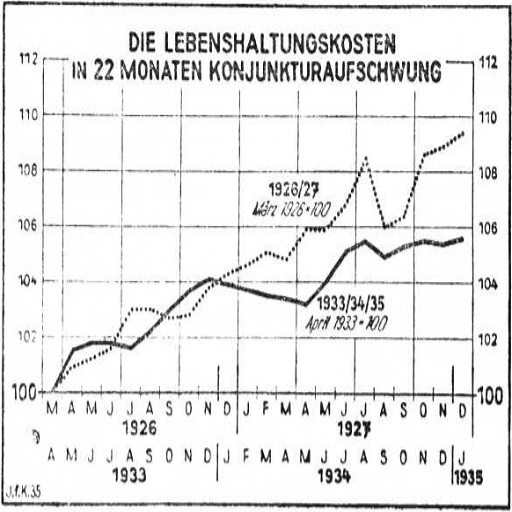
\includegraphics[width=\linewidth]{Implementation/img/alg_input.png}
        \caption{\hbadness=10000 Zu auswertendes Liniendiagramm}
        \label{fig:alg_input}
    \end{minipage}\hfill % Add space between figures
    \begin{minipage}{0.315\textwidth} % Second figure
        \centering
        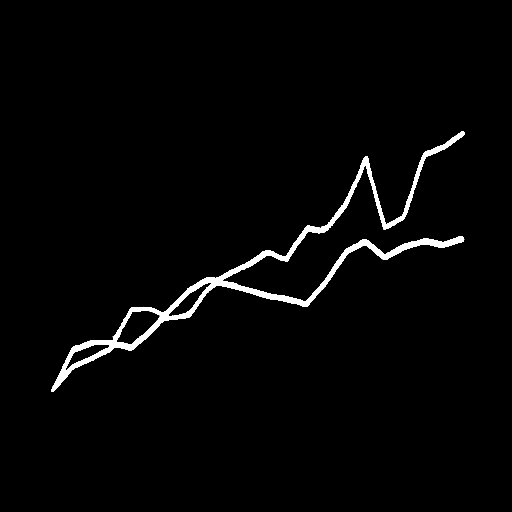
\includegraphics[width=\linewidth]{Implementation/img/alg_pred.png}
        \caption{\hbadness=10000 Semantische U-Net Vorhersage}
        \label{fig:alg_pred}
    \end{minipage}\hfill % Add space between figures
    \begin{minipage}{0.315\textwidth} % Second figure
        \centering
        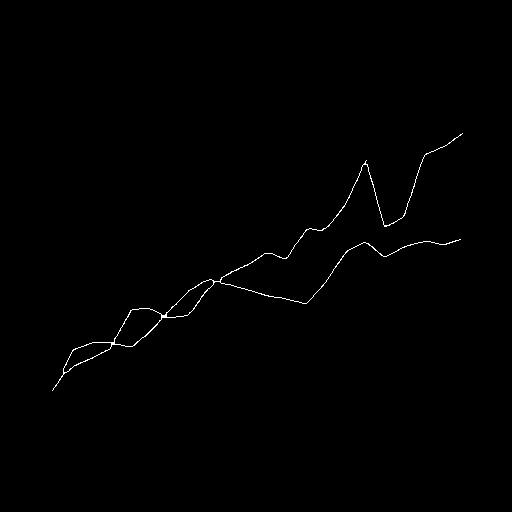
\includegraphics[width=\linewidth]{Implementation/img/alg_skeletonized.png}
        \caption{\hbadness=10000 Skelletierte Binärmaske}
        \label{fig:alg_skeletonized}
    \end{minipage}
\end{figure}

Um das Problem der Linientrennung zu überwinden wurde die Entscheidung getroffen einen primitiven Algorithmus zu verwenden, welcher die Wertelinien anhand ihrer räumlichen Position im Diagramm willkürlich differenziert. Im Folgenden werden alle sich überschneidenden Wertelinien nach dieser Approximation getrennt. Dementsprechend wurde das anspruchsvolle Problem der Wertelinientrennung im Weiteren aufgrund seiner Komplexität und des begrenzten Rahmens dieser Arbeit nicht weiter eingehend behandelt.
\\
Dieser Linientrennungsalgorithmus funktioniert wie folgt: Zuerst wird die gesamte Anzahl der Wertelinien ermittelt. Dazu wird für jede vertikale Pixelspalte des Bildes das Aufkommen von nicht-schwarzen Pixel gezählt. Da im Fall von vertikal verlaufenden Wertelinien mehrere von diesen aufeinanderfolgen können muss eine Gruppe an sequentiellen nicht-schwarzen Pixel als nur ein Aufkommen gewertet werden. Die berechneten Werte pro Pixelspalte werden daraufhin der Aufkommensgröße nach sortiert und die größten 5\% entfernt. Diese enthalten mögliche fehlerbehaftete Werte aufgrund eventueller Artefakte in der Werteliniensegmentation. Anschließend wird der verbleibende Maximalwert als gesamte Linienanzahl definiert.
\\
Nach Erhalt dieser berechneten Linienanzahl des Diagramms werden erneut alle Pixelspalten der vorhergesagten Binärmaske durchlaufen. Ebenfalls wird wieder die Anzahl der Aufkommenden Wertelinien gezählt. Besitzt die jeweilige Pixelspalte nun dieselbe Anzahl an Linien wie die berechnete gesamte Linienanzahl, dann wird die \emph{i-te} sequentielle Gruppe an nicht-schwarzen Pixel der \emph{i-ten disjunkten Wertelinienbinärmaske} zugeordnet. Sollte dies allerdings nicht der Fall sein, wird die gesamte Pixelspalte in eine \emph{gemeinsam genutzte Binärmaske} übertragen.

\begin{figure}[H] % or any other figure positioning (H, h, t, b)
    \centering
    \begin{minipage}{0.315\textwidth} % First figure
        \centering
        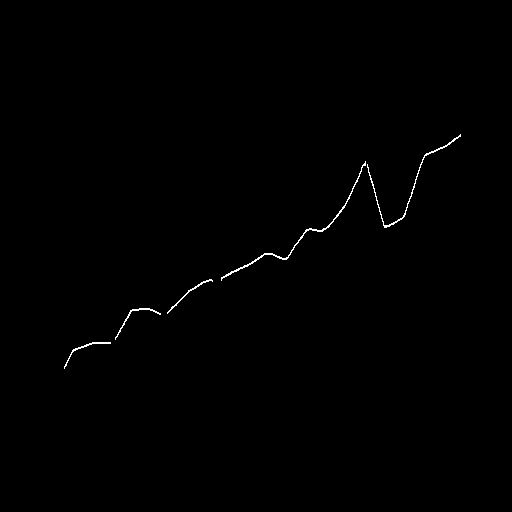
\includegraphics[width=\linewidth]{Implementation/img/alg_layer1.png}
        \caption{\hbadness=10000 Disjunkte Binärmaske der ersten Linie}
        \label{fig:alg_layer1}
    \end{minipage}\hfill % Add space between figures
    \begin{minipage}{0.315\textwidth} % Second figure
        \centering
        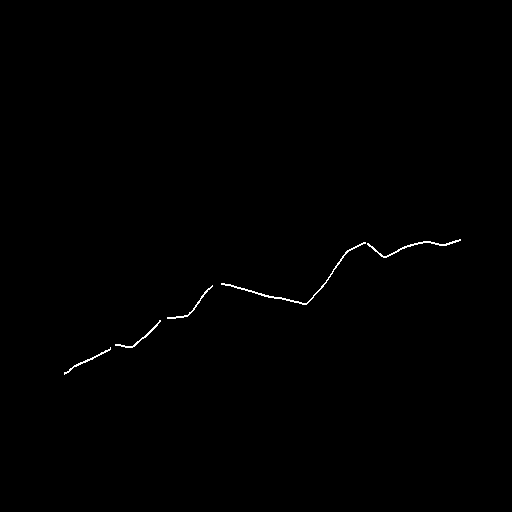
\includegraphics[width=\linewidth]{Implementation/img/alg_layer2.png}
        \caption{\hbadness=10000 Disjunkte Binärmaske der zweiten Linie}
        \label{fig:alg_layer2}
    \end{minipage}\hfill % Add space between figures
    \begin{minipage}{0.315\textwidth} % Second figure
        \centering
        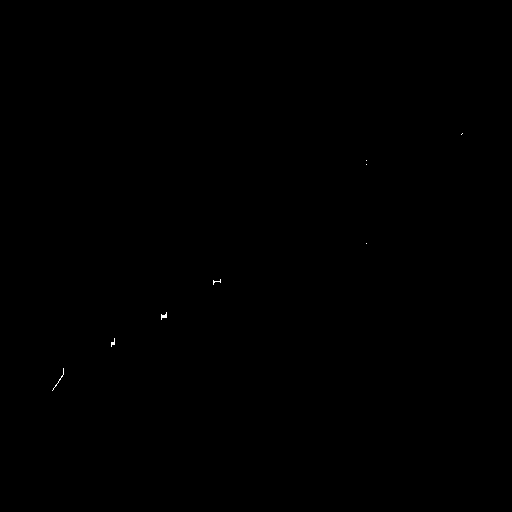
\includegraphics[width=\linewidth]{Implementation/img/alg_shared.png}
        \caption{\hbadness=10000 Gemeinsam genutzte Binärmaske}
        \label{fig:alg_shared}
    \end{minipage}
\end{figure}

Somit können die Wertelinien anhand ihrer Position differenziert werden. Um nun die einzelnen kontinuierlichen Linienwerte zu extrahieren, müssen die disjunkten Binärmasken lediglich jeweils mit der gemeinsam genutzten Maske bitweise vereinigt werden. Durch die OpenCV Funktion des Auffindens verbundener Komponenten (connected components) wird anschließend die räumlich längste ausgewählt und der Mittelwert aller nicht-schwarzen Pixel pro Pixelspalte dieser Komponente berechnet. Um möglichem Rauschen zu entgegenwirken wird nach Gaußscher Weichzeichnung (gaussian blur) mit einem Kern von 5x5 Pixel die Positionssequenz jeder getrennten Wertelinie im Diagramm ermittelt.

\begin{figure}[H] % or any other figure positioning (H, h, t, b)
    \centering
    \begin{minipage}{0.315\textwidth} % First figure
        \centering
        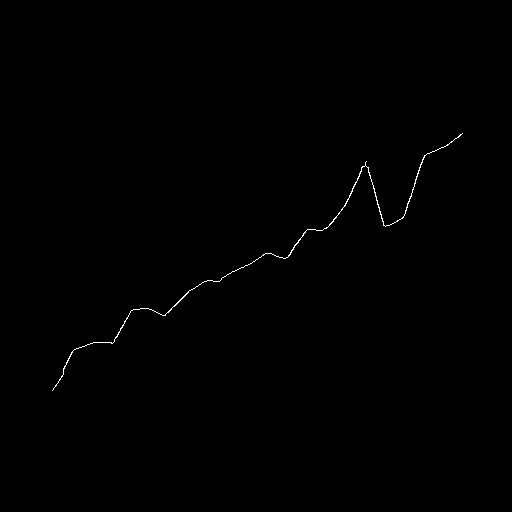
\includegraphics[width=\linewidth]{Implementation/img/alg_layer1_processed.png}
        \caption{\hbadness=10000 Vereinigte Binärmaske der ersten Linie}
        \label{fig:alg_layer1_processed}
    \end{minipage}\hfill % Add space between figures
    \begin{minipage}{0.315\textwidth} % Second figure
        \centering
        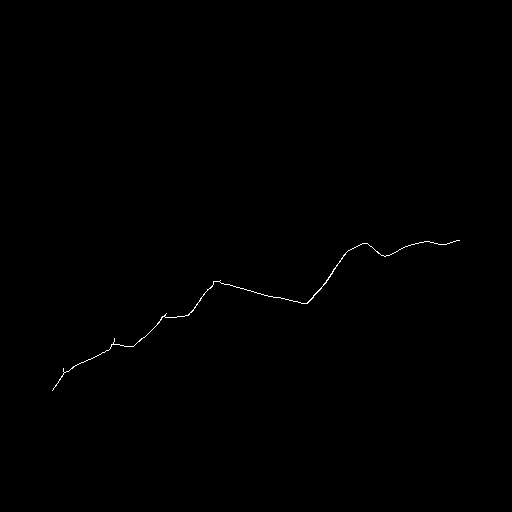
\includegraphics[width=\linewidth]{Implementation/img/alg_layer2_processed.png}
        \caption{\hbadness=10000 Vereinigte Binärmaske der zweiten Linie}
        \label{fig:alg_layer2_processed}
    \end{minipage}\hfill % Add space between figures
    \begin{minipage}{0.315\textwidth} % Second figure
        \centering
        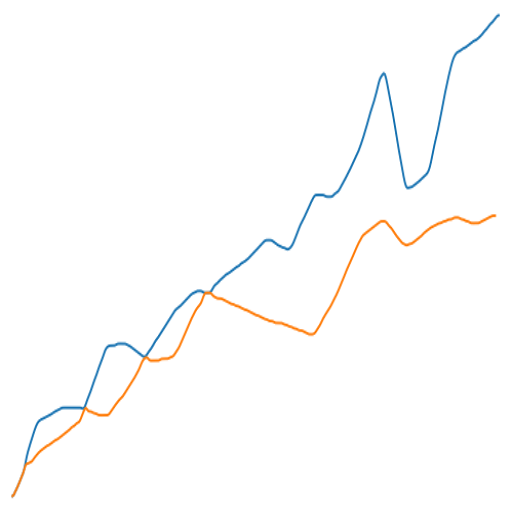
\includegraphics[width=\linewidth]{Implementation/img/alg_mat.png}
        \caption{\hbadness=10000 Getrennte Wertelinien}
        \label{fig:alg_mat}
    \end{minipage}
\end{figure}

\subsection{Achsenerkennung durch optischer Schriftzeichenerkennung}

Der andere Teil der Liniendiagrammsauswertung setzt sich aus optischen Schriftzeichenerkennung zusammen, aus welcher Titel, Linienbezeichnungen und Achsenbeschriftungen (label) ausgearbeitet werden können. Für die Label der Achsen wird außerdem derer Mittelpunktposition im Diagramm für die numerische Tabellenformauswertung verwendet. Bis auf limitierte Ausnahmen befinden sich so alle Datenpunkte, beispielweise bei Diagramme über Jahresentwicklungen, in der Jahresmitte.
\\
Für die optische Schriftzeichenerkennung wurde die JavaScript Bibliothek Chrome Lens OCR \cite{dimden2024chromelensocr} verwendet, während der restliche Algorithmus weiterhin in Python implementiert wurde. Diese OCR-Bibliothek verwendet die im Chromium Browser eingebettete Google Lens OCR und kann ohne weiteren Authentifizierungsprozess genutzt werden, weshalb sich für sie entschieden wurde. Die Brücke zwischen Python und JavaScript erfolgt durch das programmatische Aufrufen des JavaScript Codes über die Konsole in Python, welcher daraufhin von ihr in Textform ausgelesen und verarbeitet werden kann. Zur Verfügung gestellt werden die erkannten Textbezeichnungen selbst, aber auch ihre jeweiligen absoluten und relativen Positionen innerhalb des Diagrammbilds.
\\
Nach dem alle erkannten OCR-Labels bereitgestellt wurden, werden diese mithilfe ihrer Mittelpunktpositionen in fünf disjunkte Gruppen eingeteilt: Titel, Linienbezeichnungen, linke Y-Achse, rechte Y-Achse und untere X-Achse.

\begin{figure}[H]
    \centering
    \captionsetup{width=.75\linewidth}
    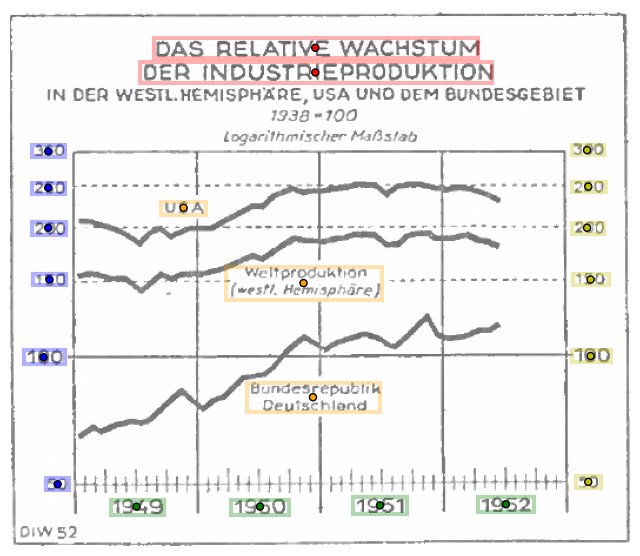
\includegraphics[width=.75\textwidth]{Implementation/img/ocr.png}
    \caption{\hbadness=10000 Zuordnung der erkannten Textbeschriftungen in die fünf disjunkte Gruppen samt ihrer jeweiligen Mittelpunktpositionen}
    \label{fig:ocr}
\end{figure}

Für die drei Achsenbeschriftungen werden nur jenige Labels untersucht, welche sich auf dem äußeren Rand von 15\% des Bildes befinden. Die horizontale und vertikale Mittelwertposition aller Labels für die drei Achsen wird bestimmt und mit dieser werden mögliche Beschriftungen, welche sich nicht innerhalb 2\% der jeweiligen Mittelwertlinie befinden, aussortiert. Ebenfalls werden alle Beschriftungen unterhalb der erkannten X-Achse, unabhängig dieser vorherigen Einschrenkung, ignoriert. Um mögliche Schriftzeichenerkennungsfehler entgegenzuwirken wird der Text der erkannten Achsenlabels gefiltert. Erkannte Kommas werden in Punkte verwandelt und danach alle Buchstaben und andere Zeichen entfernt, sodass der Text am Ende nur noch aus den Zeichen 0-9, Punkte und Minuszeichen besteht. Diese Entscheidung wurde getroffen um fälschlicherweise miterkannte Einheitsangaben, oder andere OCR-Fehler zu verbessern. Das Aufkommen von falscher OCR bei Ziffern, z.B. die Erkennung von einem B statt einer 8, kam nur sehr selten vor, weshalb dieser Schritt gewählt wurde.
Um den Diagrammstitel zu extrahieren werden die oberen Labels ausgewählt, die sich in horizontaler Mitte befinden. Für die Wertelinienbeschriftungen werden alle Textbezeichnungen in Auswahl gezogen, welche sich innerhalb des definierten Diagrammsrand befinden. Zur Lösung des aufkommenden Minimum-Distanz-Problems werden in Verbindung mit den getrennten Wertelinienmasken aus dem vorherigen Schritt diese Labels den jeweilig nächsten Linien mithilfe der Ungarischen Methode bestmöglich zugeordnet.
\clearpage
\subsection{Grafische Darstellung und tabellarische Auswertung}

Im Anschluss der Wertelinien- und Achsenbeschriftsextraktion kann das zu auswertende Liniendiagramm visualisiert und in Tabellenform ausgewertet werden. Für die grafische Darstellung wurde die Datenvisualisierungsbibliothek Matplotlib \cite{Hunter:2007} verwendet.

\begin{figure}[H]
    \centering
    \captionsetup{width=.75\linewidth}
    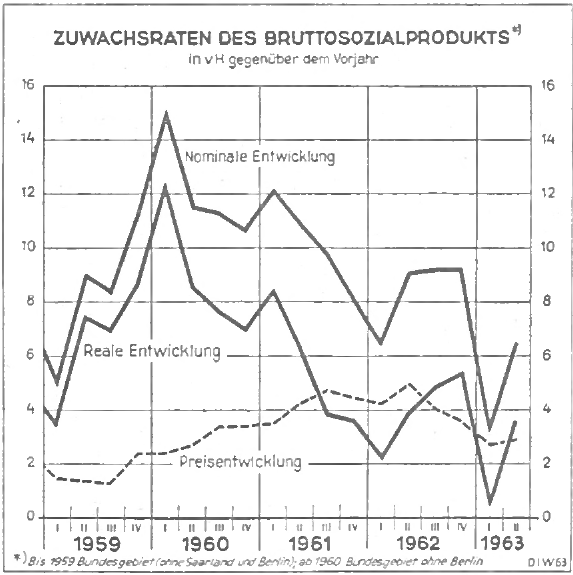
\includegraphics[width=.75\textwidth]{Implementation/img/extraction_input2.png}
    \caption{\hbadness=10000 Zu auswertendes Liniendiagramm}
    \label{fig:extraction_input}
\end{figure}

Die extrahierten kontinuierlichen Linienwerte können nach vorherigem Skalieren, basierend auf der Bildgröße des Diagramms durch Matplotlib dargestellt werden. Jeder dieser Linien kann ein Bezeichnung zugeordnet werden, welche in der Legende aufgezählt wird. Zudem kann der Titel des Graphs (plot) gesetzt werden. Die Position der jeweiligen Achsenticks kann, wie vermerkt, durch die Mittelpunktpositionen der einzelnen eingeteilten Achsenbeschriftungen eingestellt werden, sowie deren jeweilige Labels. Pro X-Achsen Label wurde außerdem eine vertikale, gestrichelte Linie visualisert.

\begin{figure}[H]
    \centering
    \captionsetup{width=.75\linewidth}
    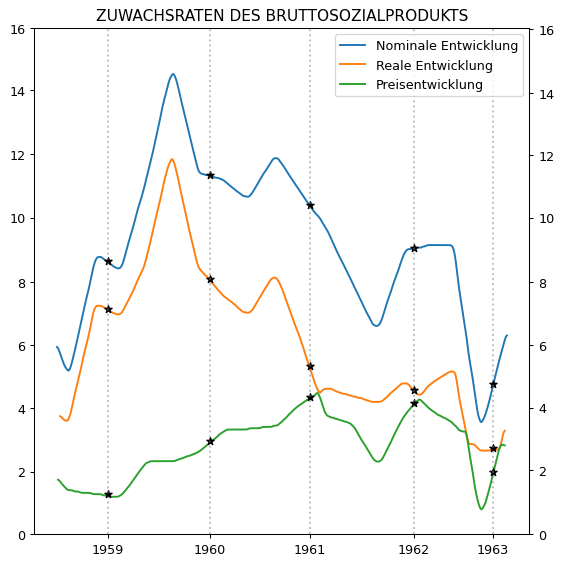
\includegraphics[width=.75\textwidth]{Implementation/img/extraction_output2.png}
    \caption{\hbadness=10000 Durch Matplotlib visualisertes, extrahiertes Liniendiagramm}
    \label{fig:extraction_output}
\end{figure}

Die eigentliche numerische Auswertung erfolgt nun ohne weiteren großen Aufwand. Für jedes Label der X-Achse wird dessen Schnittpunkt einer von ihrem Mittelpunkt aus verlaufenden, vertikalen Linie mit allen Werteliniensequenzen berechnet und der die räumliche Y-Position bestimmt. Anschließend wurde durch linearer Inter- und Extrapolation mithilfe der SciPy \cite{2020SciPy-NMeth} Bibliothek der genaue Y-Wert zwischen den Labelwerten der linken Y-Achse berechnet. Zu notieren ist hier, dass diese lineare Interpolation bei Diagrammen mit beispielsweise logarithmischer Skala zu Evaluationsfehlern führt. Diese Diagrammsform ist jedoch so gering vorkommend, weshalb diese fehlerbehaftete Herangehensweise akzeptabel erscheint. Zu visuellem Zweck wurden diese Schnittpunkte ebenfalls in dem grafisch dargestellten Graph veranschaulicht.

\begin{table}[H]
    \centering
    \begin{tabular}{|l|l|l|l|l|l|}
        \hline
        \rowcolor[HTML]{EFEFEF}
                             & 1959 & 1960  & 1961  & 1962 & 1963 \\ \hline
        Nominale Entwicklung & 8.63 & 11.33 & 10.39 & 9.04 & 4.73 \\ \hline
        Reale Entwicklung    & 7.12 & 8.08  & 5.29  & 4.53 & 2.70 \\ \hline
        Preisentwicklung     & 1.23 & 2.91  & 4.32  & 4.14 & 1.94 \\ \hline
    \end{tabular}
    \caption{Ausgewertetes Liniendiagrammen in Tabellenform}
\end{table}
